\documentclass[tikz,border=5pt]{standalone}
\usepackage{ctex,amsmath}
\usetikzlibrary{arrows.meta,calc,decorations.markings}
\tikzset{>=Latex,branch/.style={blue!65!black,thick,
 postaction={decorate},decoration={markings,mark=at position .66 with {\arrow{Latex}}}},
 nodepoint/.style={circle,fill=black,inner sep=1.5pt},guide/.style={gray!60,dashed}}
% 箭头始终只代表正极至负极的参考方向；负支路电流不翻转本图箭头。
\newcommand{\heptagon}{
 \foreach \i in {0,...,6}{
  \pgfmathsetmacro{\theta}{115.7142857-51.4285714*\i}
  \coordinate (n\i) at (\theta:1.65);
  \node[nodepoint] at(n\i){};
  \node at(\theta:2.02){$A_{\i}$};}}
\begin{document}
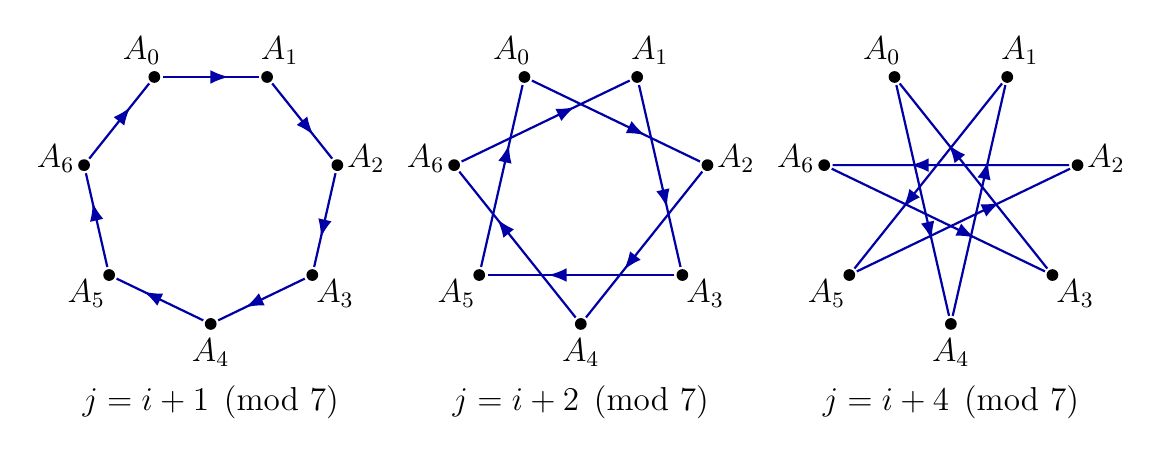
\begin{tikzpicture}[font=\large]
 \foreach \d/\shift in {1/0,2/4.7,4/9.4}{
  \begin{scope}[xshift=\shift cm]
   \heptagon
   \foreach \i in {0,...,6}{
    \pgfmathtruncatemacro{\j}{mod(\i+\d,7)}
    \draw[branch,shorten >=3pt,shorten <=3pt](n\i)--(n\j);
   }
   \node at(0,-2.65){$j=i+\d\pmod 7$};
  \end{scope}
 }
\end{tikzpicture}
\begin{tikzpicture}[font=\large]
 \coordinate (a) at(-3,0);\coordinate (b) at(3,0);
 \fill(a)circle(.045)node[left]{$A_i,\ V_i$};
 \fill(b)circle(.045)node[right]{$A_j,\ V_j$};
 \draw[thick](a)--(-.48,0)(.43,0)--(b);
 \draw[thick,fill=blue!8](-.48,-.43)--(-.48,.43)--(.43,0)--cycle;
 \draw[very thick](.43,-.49)--(.43,.49);
 \draw[blue!65!black,thick,->](-1.35,.92)--(1.45,.92)
  node[midway,above]{$I_{ij}=I_0(\mathrm e^{\alpha U_{ij}}-1)$};
 \node[below]at(-1.6,-.5){正极};\node[below]at(1.6,-.5){负极};
 \node at(0,-1.65){$U_{ij}=V_i-V_j$};
\end{tikzpicture}
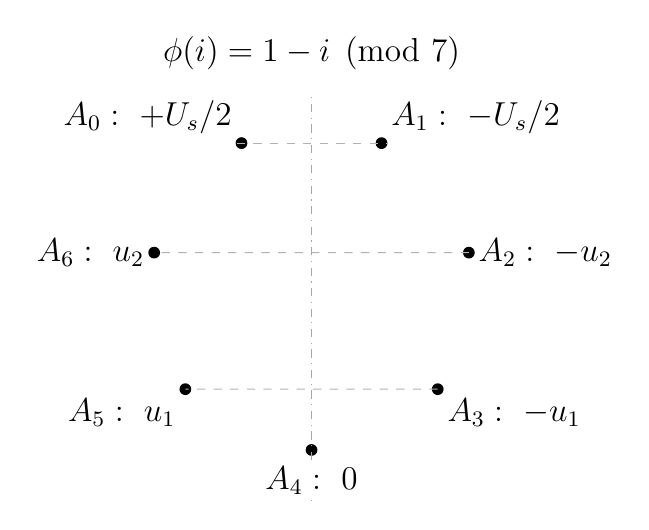
\begin{tikzpicture}[font=\large]
 \foreach \i in {0,...,6}{
  \pgfmathsetmacro{\theta}{115.7142857-51.4285714*\i}
  \coordinate (n\i) at (\theta:2.05);
  \node[nodepoint] at(n\i){};
 }
 \draw[guide](-.95,1.847)--(.95,1.847);
 \draw[guide](n2)--(n6)(n3)--(n5);
 \draw[gray!70,dash dot](0,-2.7)--(0,2.5);
 \node[above left]at(n0){$A_0:\ +U_s/2$};
 \node[above right]at(n1){$A_1:\ -U_s/2$};
 \node[right]at(n2){$A_2:\ -u_2$};
 \node[below right]at(n3){$A_3:\ -u_1$};
 \node[below=4pt,fill=white,inner sep=2pt]at(n4){$A_4:\ 0$};
 \node[below left]at(n5){$A_5:\ u_1$};
 \node[left]at(n6){$A_6:\ u_2$};
 \node[above]at(0,2.65){$\phi(i)=1-i\pmod 7$};
\end{tikzpicture}
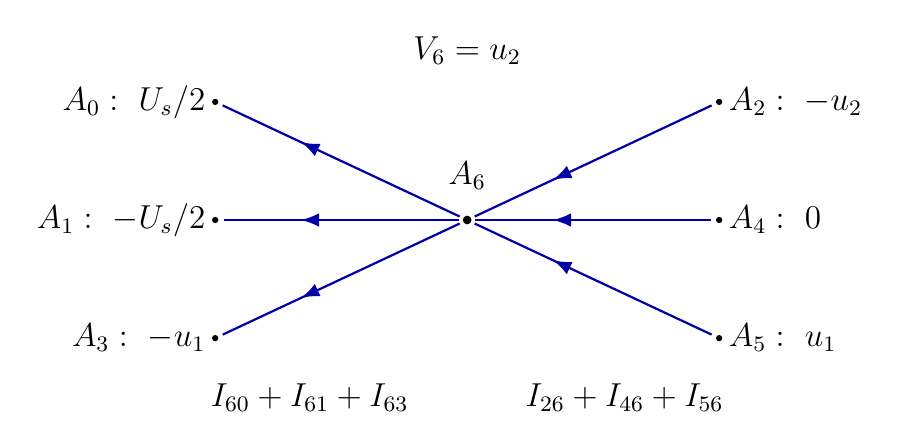
\begin{tikzpicture}[font=\large]
 \coordinate (c) at(0,0);
 \foreach \y/\i/\v in {1.5/0/{U_s/2},0/1/{-U_s/2},-1.5/3/{-u_1}}{
  \coordinate (l\i) at(-3.2,\y);
  \draw[branch,shorten >=3pt,shorten <=3pt](c)--(l\i);
  \fill(l\i)circle(.04)node[left]{$A_{\i}:\ \v$};
 }
 \foreach \y/\i/\v in {1.5/2/{-u_2},0/4/{0},-1.5/5/{u_1}}{
  \coordinate (r\i) at(3.2,\y);
  \draw[branch,shorten >=3pt,shorten <=3pt](r\i)--(c);
  \fill(r\i)circle(.04)node[right]{$A_{\i}:\ \v$};
 }
 \fill(c)circle(.055);
 \node[above,inner sep=1pt]at(0,.35){$A_6$};
 \node at(0,2.15){$V_6=u_2$};
 \node at(-2,-2.25){$I_{60}+I_{61}+I_{63}$};
 \node at(2,-2.25){$I_{26}+I_{46}+I_{56}$};
\end{tikzpicture}
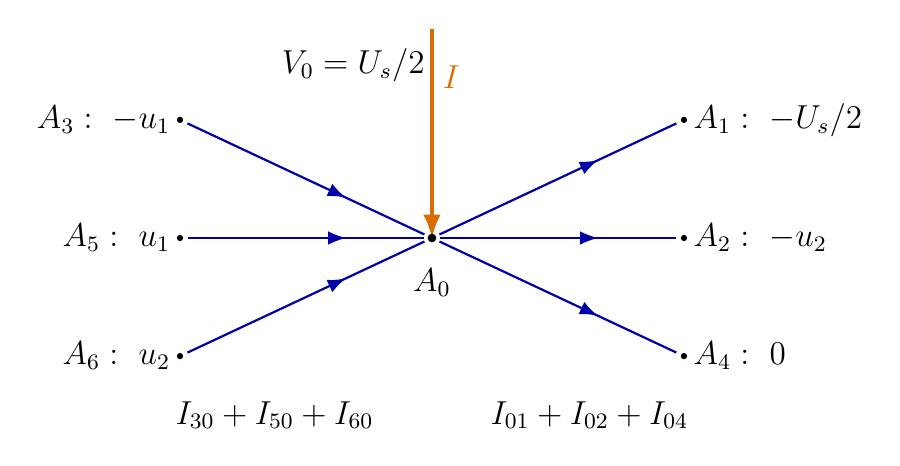
\begin{tikzpicture}[font=\large]
 \coordinate (c) at(0,0);
 \foreach \y/\i/\v in {1.5/1/{-U_s/2},0/2/{-u_2},-1.5/4/{0}}{
  \coordinate (r\i) at(3.2,\y);
  \draw[branch,shorten >=3pt,shorten <=3pt](c)--(r\i);
  \fill(r\i)circle(.04)node[right]{$A_{\i}:\ \v$};
 }
 \foreach \y/\i/\v in {1.5/3/{-u_1},0/5/{u_1},-1.5/6/{u_2}}{
  \coordinate (l\i) at(-3.2,\y);
  \draw[branch,shorten >=3pt,shorten <=3pt](l\i)--(c);
  \fill(l\i)circle(.04)node[left]{$A_{\i}:\ \v$};
 }
 \draw[orange!85!black,very thick,->](0,2.65)--(c)
  node[pos=.23,right]{$I$};
 \fill(c)circle(.055);
 \node[below,inner sep=1pt]at(0,-.35){$A_0$};
 \node at(-1.0,2.2){$V_0=U_s/2$};
 \node at(-2,-2.25){$I_{30}+I_{50}+I_{60}$};
 \node at(2,-2.25){$I_{01}+I_{02}+I_{04}$};
\end{tikzpicture}
\end{document}
